\section{Community Detection}
Party systems can be characterized based on their fragmentation and polarization. Party fragmentation corresponds to the number of parties existing in a political system, while polarization is related to the multiple opinions that lead to the division of members into groups with distinct political ideologies.\\
It's not uncommon that in fragmented systems the multiple political parties often make coalitions, or alliances, to reach a common end. Thus, a great amount of ideological similarity, expressed by the voting decisions, is observed across different parties, generating ideological communities \cite{AnIdeoComm}.\\

\begin{table*}[h]
\begin{tabular}{c|cccc|ccccc|ccccc|}
\cline{2-15}
                                 & \multicolumn{4}{c|}{\textbf{Louvain}} & \multicolumn{5}{c|}{\textbf{Angel}} & \multicolumn{5}{c|}{\textbf{K-Clique}} \\ \hline
\multicolumn{1}{|c|}{\textbf{Year}} &
  \textbf{\begin{tabular}[c]{@{}c@{}}\# of \\      Comm.\end{tabular}} &
  \textbf{Mod.} &
  \textbf{\begin{tabular}[c]{@{}c@{}}Avg.\\      PD\end{tabular}} &
  \textbf{\begin{tabular}[c]{@{}c@{}}SD\\      PD\end{tabular}} &
  \textbf{\begin{tabular}[c]{@{}c@{}}Merging \\ Thr.\end{tabular}} &
  \textbf{\begin{tabular}[c]{@{}c@{}}\# of \\      Comm.\end{tabular}} &
  \textbf{Mod.} &
  \textbf{\begin{tabular}[c]{@{}c@{}}Avg.\\      PD\end{tabular}} &
  \textbf{\begin{tabular}[c]{@{}c@{}}SD\\      PD\end{tabular}} &
  \textbf{K} &
  \textbf{\begin{tabular}[c]{@{}c@{}}\# of \\      Comm.\end{tabular}} &
  \textbf{Mod.} &
  \textbf{\begin{tabular}[c]{@{}c@{}}Avg.\\      PD\end{tabular}} &
  \textbf{\begin{tabular}[c]{@{}c@{}}SD\\      PD\end{tabular}} \\ \hline
\multicolumn{1}{|c|}{2013}       & 4     & 0.21     & 0.74     & 0.14    & 0      & 4  & 0.21  & 0.74  & 0.14  & 2     & 4   & 0.21   & 0.74   & 0.14   \\
\multicolumn{1}{|c|}{2014}       & 4     & 0.21     & 0.73     & 0.11    & 0      & 3  & 0.20  & 0.75  & 0.13  & 3     & 4   & 0.20   & 0.73   & 0.13   \\
\multicolumn{1}{|c|}{2015}       & 3     & 0.20     & 0.70     & 0.11    & 0.21   & 3  & 0.20  & 0.70  & 0.11  & 4     & 3   & 0.20   & 0.70   & 0.11   \\
\multicolumn{1}{|c|}{2016}       & 4     & 0.15     & 0.68     & 0.13    & 0      & 3  & 0.14  & 0.65  & 0.12  & 2     & 4   & 0.15   & 0.68   & 0.13   \\
\multicolumn{1}{|c|}{2017}       & 3     & 0.23     & 0.69     & 0.11    & 0.64   & 3  & 0.20  & 0.69  & 0.10  & 13    & 3   & 0.23   & 0.69   & 0.11   \\
\multicolumn{1}{|c|}{2018-xvii}  & 3     & 0.24     & 0.69     &         & *      & *  & *     & *     & *     & 11    & 4   & 0.01   & 0.67   & 0.27   \\
\multicolumn{1}{|c|}{2018-xviii} & 2     & 0.41     & 0.70     & 0.13    & 0.07   & 2  & 0.41  & 0.70  & 0.13  & 3     & 2   & 0.41   & 0.72   & 0.13   \\
\multicolumn{1}{|c|}{2019}       & 3     & 0.25     & 0.70     & 0.14    & 0.93   & 2  & 0.11  & 0.70  & 0.14  & 2     & 1   & 0      & 0.70   & 0.14   \\
\multicolumn{1}{|c|}{2020}       & 2     & 0.46     & 0.72     & 0.14    & 0.07   & 2  & 0.46  & 0.71  & 0.14  & 3     & 2   & 0.46   & 0.71   & 0.14   \\
\multicolumn{1}{|c|}{2021}       & 2     & 0.27     & 0.68     & 0.13    & 1      & 1  & 0.11  & 0.67  & 0.11  & 2     & 2   & 0.02   & 0.68   & 0.13   \\
\multicolumn{1}{|c|}{2022}       & 2     & 0.22     & 0.75     & 0.10    & 1   & 2  & 0.03  & 0.71 & 0.10  & *     & *   & *      & *      & *      \\ \hline
\end{tabular}
\caption{Community detection results obtained for different algorithms. Note: we couldn't calculate the values marked by * due to problems in the convergence of algorithms.}
\label{tab:community}
\end{table*}


Table \ref{tab:community} shows the results of different community detection algorithms on the yearly networks. The algorithms adopted for the search of communities were Louvain, Angel, and K-clique.\\

We decided to use different algorithms to exploit the differences between the communities found, since each algorithm has its definition of community.\\

After a very quick tuning phase, we decided to set the merging threshold of Angel independently for each year. We defined some candidates values, $\{0, 0.07, 0.14, 0.21, 0.28, 0.35,\\ 0.42, 0.5, 0.57, 0.64, 0.71, 0.78, 0.85, 0.92, 1\}$, and selected the value associated to the highest modularity. We also ignored the communities with less than $4$ nodes. \\

Similarly, for the k-clique algorithm we decided to range the size from $2$ to $15$ and select, for each network, the value associated with the highest modularity score.\\

We decide to use the modularity score to evaluate the communities structure, and an external measure that fits our case study, the \textit{Partisan Discipline} metric \cite{PD}.
 This metric captures the ideological alignment of a member to his party (or his community). Given a member \textit{x}, the \textit{Partisan Discipline} of \textit{x} is given by the fraction of all voting sessions where \textit{x} voted in the same way as the majority of the member in his party (or his community). 
\begin{equation}
    p = \dfrac{\sum_{i = 1}^{n}{I(x, p_{x,i})}} {n}
\end{equation}

\noindent Where $I(x, p_{x,i})$ is 1 if \textit{x} voted in the same ways as its party (or community) in the same voting session, $0$ otherwise, and \textit{n} is the total number of voting sessions.
 It can range from 0 to 1, where 1 indicates that a member is cohesive and 0 otherwise.\\

A common result between the algorithms is the fact that the number of communities found is always much smaller than the total number of parties, which is $12$ before $2017$, $10$ after, confirming the fragmentation and ideological overlap of multiple parties.\\

\begin{table}[h]
\begin{tabular}{ccclll}
\multicolumn{1}{c|}{Party}    & Community 1          & Community 2          &  &  &  \\ \cline{1-3}
\multicolumn{1}{c|}{SI}       & 0.05                 & 0                    &  &  &  \\
\multicolumn{1}{c|}{CI}       & 0.02                 & 0                    &  &  &  \\
\multicolumn{1}{c|}{PD}       & 0.23                 & 0                    &  &  &  \\
\multicolumn{1}{c|}{IPF-IC}   & 0.06                 & 0                    &  &  &  \\
\multicolumn{1}{c|}{M5S}      & 0.40                 & 0.01                 &  &  &  \\
\multicolumn{1}{c|}{IV-IC'E'} & 0.07                 & 0                    &  &  &  \\
\multicolumn{1}{c|}{LEGA}     & 0                    & 0.50                 &  &  &  \\
\multicolumn{1}{c|}{FI}       & 0.01                 & 0.25                 &  &  &  \\
\multicolumn{1}{c|}{FDI}      & 0                    & 0.18                 &  &  &  \\
\multicolumn{1}{c|}{MISTO}    & 0.16                 & 0.06                 &  &  &  \\
\multicolumn{1}{l}{}          & \multicolumn{1}{l}{} & \multicolumn{1}{l}{} &  &  & 
\end{tabular}
\caption{Proportion of political parties member inside the different communities extracted using Louvain algorithm for the 2020 voting sessions.}
\label{tab:community_party}
\end{table}

The average \textit{Partisan Discipline} of these communities is very close, or slightly worse, to the average computed using the original parties. Also, the standard deviation of the \textit{Partisan Discipline} is almost every time lower in the communities than in original parties. Overall, members are disciplined with respect to the voting preferences of the parties, and the resulting communities are quite cohesive in their voting patterns. \\

In contrast, the topological structure of the identified communities, expressed with the \textit{modularity} score, is in general weak.\\ Independently from the algorithm used, in $2020$ the communities have the highest modularity, a moderate value that tells us that there is a discernible separation between communities in terms of their internal connectivity. We may hypothesize that this can be related to the Covid-19 emergency, which created a stronger distinction between communities.\\
Then, starting from the following year, the modularity decreases, stabilizing itself with similar values of the previous years using Louvain, while using Angel and K-clique the values fall and reach almost zero, indicating similarities across members of different communities.\\
This happens despite the moderately large average party discipline maintained by the communities. 

That is, the two selected metrics (Modularity and average PD) provide different views of the political scenario.\\



In general, the communities found with Angel and K-clique vary in \textit{modularity} more than the ones found with Louvain, and with both algorithms we found at least a network with a single community. With Louvain, instead, we have a more stable situation, where the number of communities doesn't affect the \textit{modularity}, which is stable around $0.2$ in most of the cases.\\

It is interesting to study how the identified communities are composed in terms of political parties. In table \ref{tab:community_party} we consider, as an example, the year 2020, where the Louvain algorithm identifies 2 distinct communities. We analyze what political parties compose these coalitions, and in what proportion.\\
The distinction between the center-left and the center-right block is evident, with a virtually negligible overlap.\\ 

To sum up, in our study we found that several parties can be grouped in few communities, characterized by disciplined members. The topological strength of communities, represented by the modularity score, is moderate, and depends on the year considered. The cohesiveness of identified communities, expressed by the average party discipline, is high and tends to remain more stable.


\section{Stream Graph}

The network we are studying is very dynamic. Opinions may change over time, and different coalitions may emerge between members of the Chamber. The changes in voting behavior may have different origins, and thus they can emerge in different timescales.\\
For this reason, it is useful to study our network from a \textit{Stream Graph} point of view.\\
Using the \textit{DyNetX} library, we create a stream graph using months as temporal snapshots.\\
For every month we create our snapshot network following the approach described at the beginning of the article. However, to have less variability in the number of nodes, we decided not to eliminate the \textit{"serial absent"} members.\\
There is still a slight variability in the number of nodes, due to the fact that data from certain members were missing in certain months.\\ Moreover, no data was available for some months (Jan-May 2018, Jan 22, Sept 22, and Oct 22); those months are not reported in the analysis.\\

For the XVII legislature, we end up with a stream graph with 600 nodes and 179421 interactions.
For the XVIII, we have a total of 615 nodes and 188783 interactions.\\

To analyze the stability of the temporal graph, we focus on monthly temporal snapshots, studying the following features evolving over time:
\begin{itemize}
    \item Number of Nodes and  Interactions (Figure \ref{fig:dynamic_nodes_edges})
    \item Average Clustering Coefficient and Average Degree (Figure \ref{fig:cc_deg})    
    \item Number of communities identified using Louvain and corresponding modularity (Figure \ref{fig:dynamic_louvain})
    \item  Average Party Discipline (Figure \ref{fig:dynamic_apd})
\end{itemize}

\begin{figure*}[h]
  \centering
  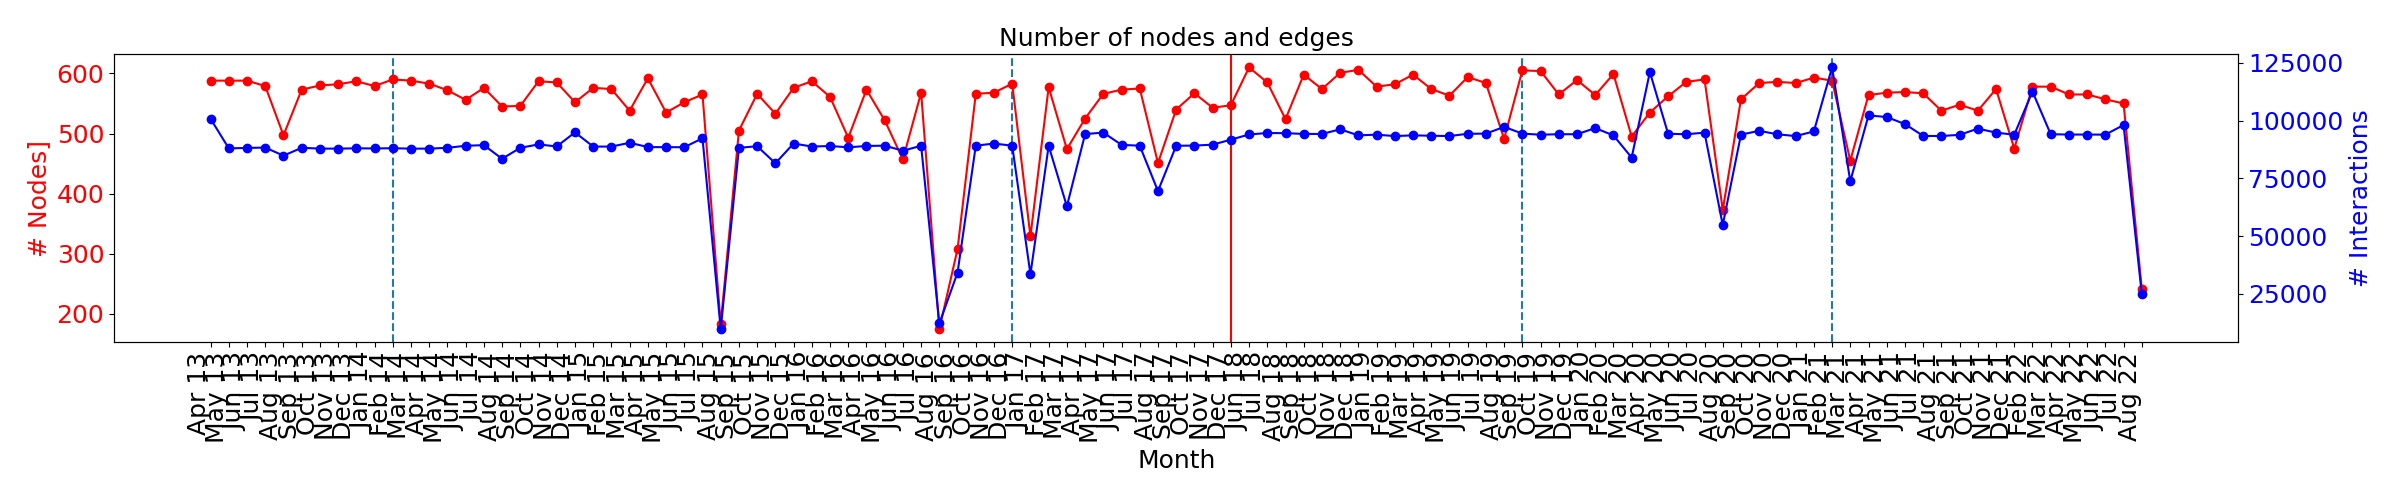
\includegraphics[width=\linewidth]{img/dynamic_nodes_edges_tot.png}
  \caption{Number of Nodes (red) and Interactions (blue) across different months of XVII and XVIII legislatures.}
  \label{fig:dynamic_nodes_edges}
\end{figure*}



\begin{figure*}[h]
  \centering
  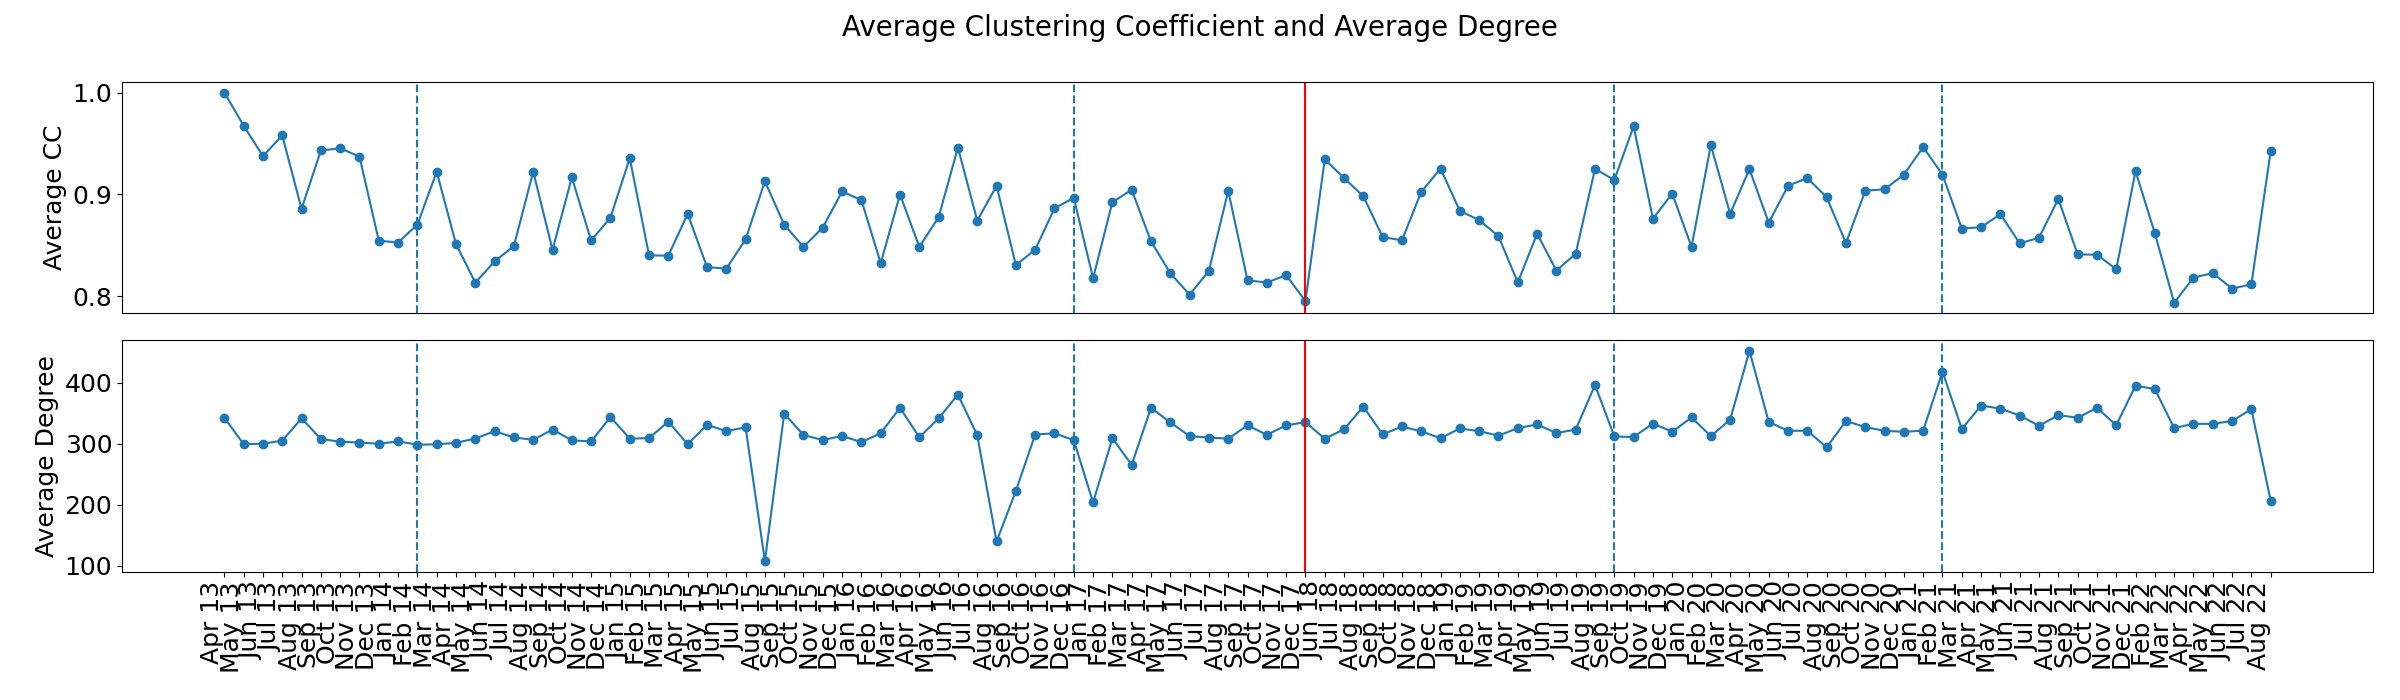
\includegraphics[width=\linewidth]{img/dynamic_avg_cc_deg_tot.png}
  \caption{Average CC (top) and Average degree (bottom).}
  \label{fig:cc_deg}
\end{figure*}

\begin{figure*}[h]
  \centering
  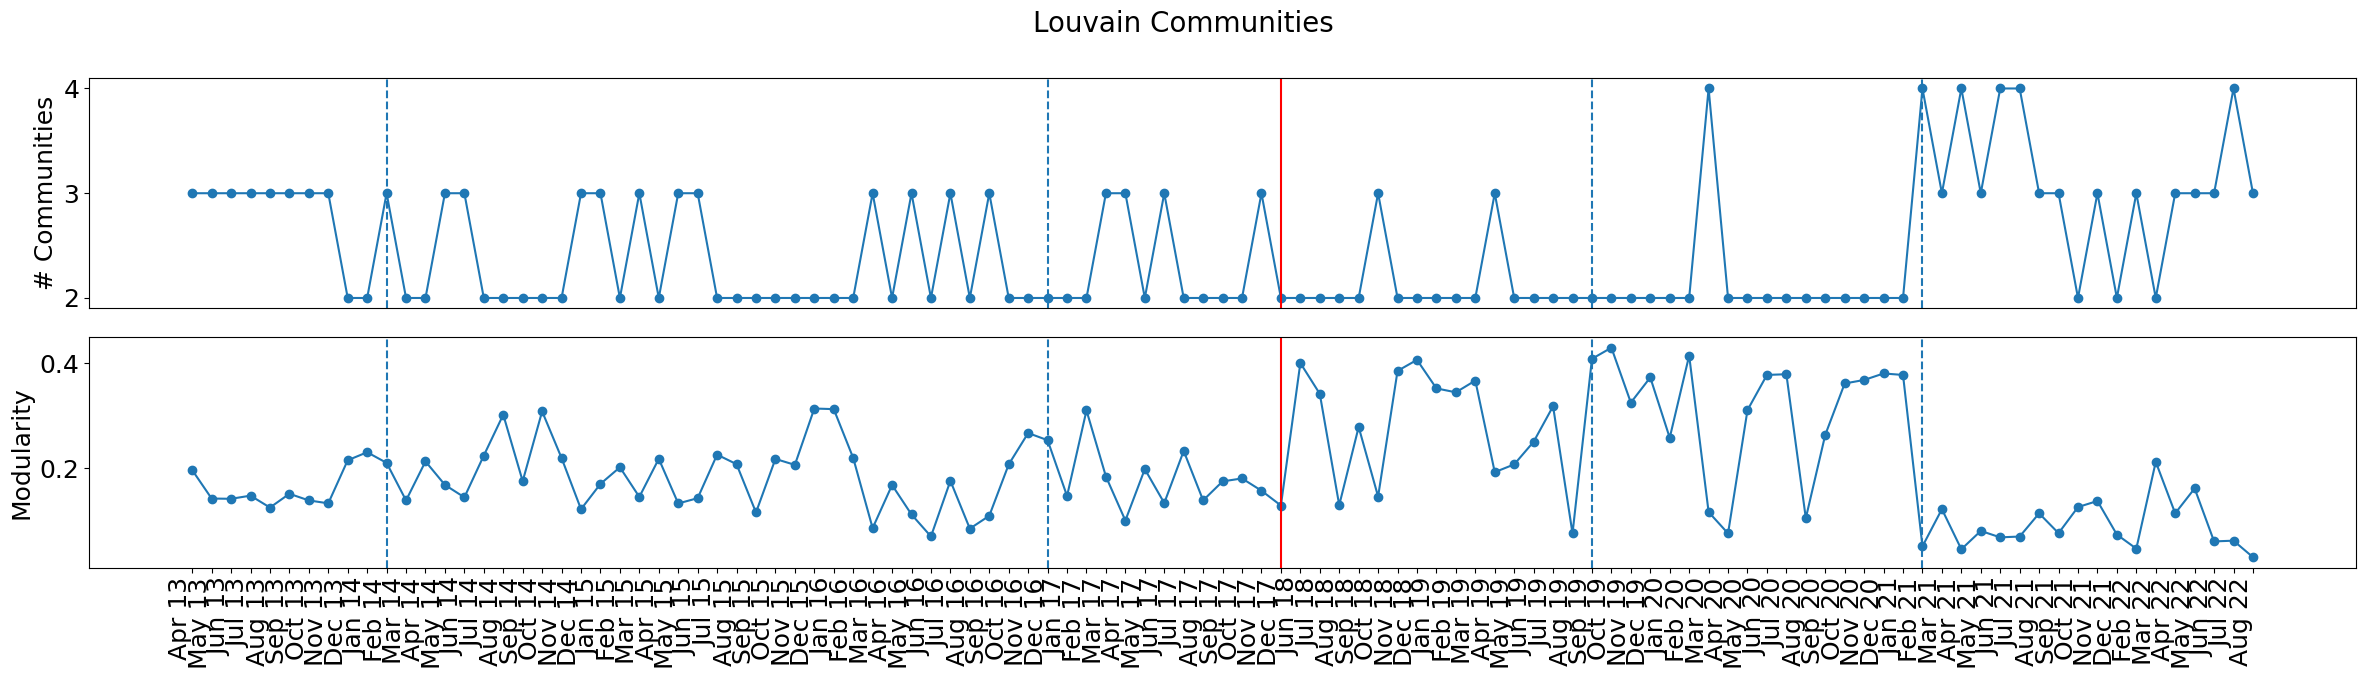
\includegraphics[width=\linewidth]{img/dynamic_louvain_tot.png}
  \caption{Number of Louvain Communities (top) and corresponding modularity (bottom).}
  \label{fig:dynamic_louvain}
\end{figure*}



\begin{figure*}[h]
  \centering
  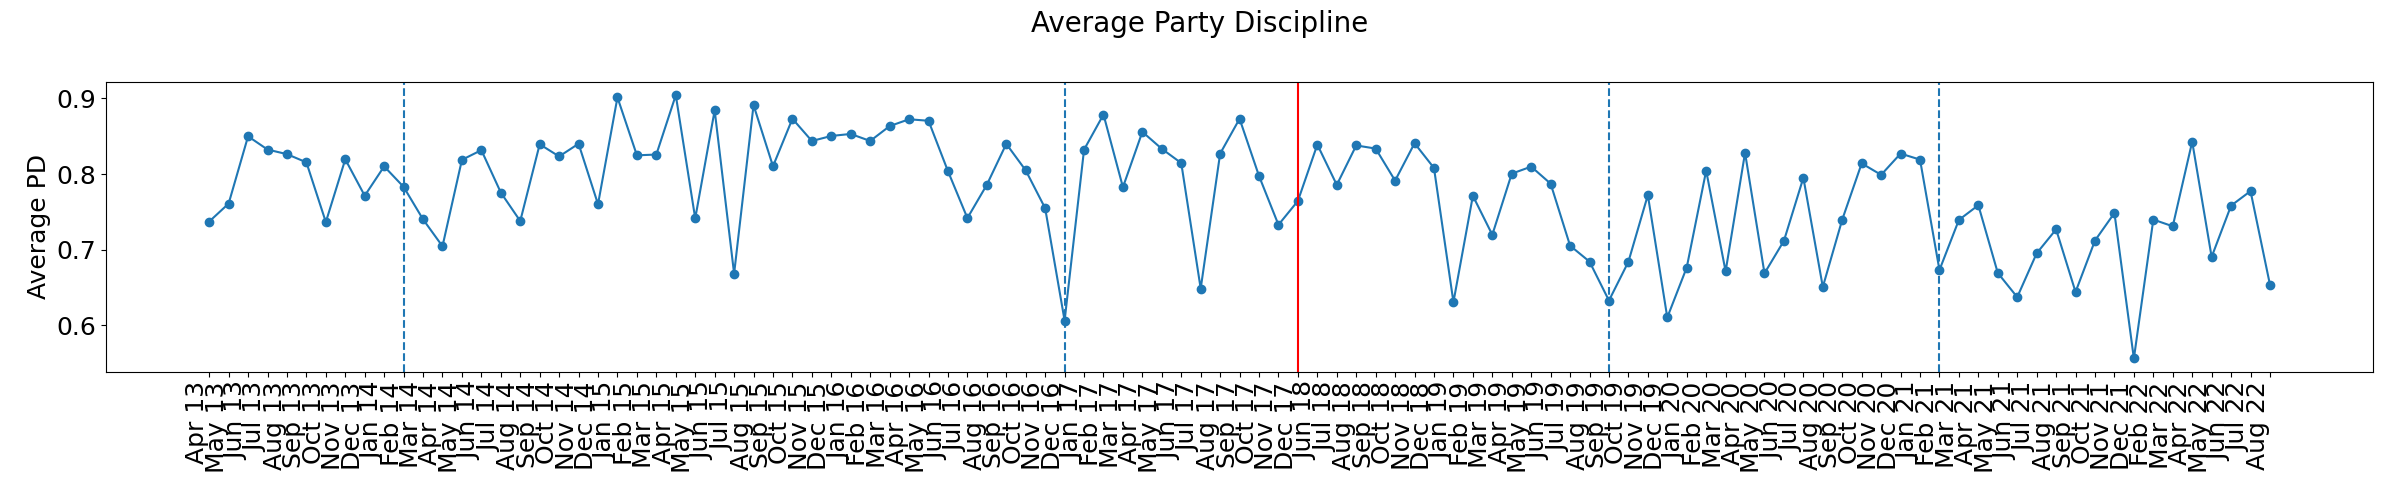
\includegraphics[width=\linewidth]{img/dynamic_apd_tot.png}
  \caption{Average Party Discipline score.}
  \label{fig:dynamic_apd}
\end{figure*}

In the figures, the vertical dashed lines correspond to months in which a new Prime Minister was appointed (and a new government formed); the red vertical line corresponds to the distinction between XVII and XVIII legislature.\\

In figure \ref{fig:dynamic_nodes_edges}, we see that the number of nodes of the network is quite stable, except for some months (typically August), where there is an evident lack of data.\\
The average number of nodes is 546, with standard deviation 77.\\
The number of edges follows a similar trend, with average 88281 and standard deviation 16621.\\
Since the average degree is the ratio between the number of edges and the number of nodes, it has a similar trend (320 $\pm$ 42).\\

The average clustering coefficient is pretty stable, showing small fluctuations across different months. In general, it has a high value (0.88 $\pm$ 0.04), indicating a high degree of clustering between members of the Chamber.\\

It is interesting to study the number of communities that are identified in different months (using Louvain). During the XVII legislature, we see that this number oscillates between 2 and 3. In the XVIII legislature, during the first two governments we almost always have a bipolar system, while during the last government the number of communities identified is more variable, ranging from 2 to 4.\\
As we have already seen with yearly data, the number of communities identified is smaller than the number of actual parties present in the Chamber. This highlights the ideological overlap of some parties.\\

The modularity score is a great indicator of how strong the communities found are from a topological point of view.
 Modularity computed over the Louvain communities shows a great variability: across all the months considered, it has a mean of 0.2 and a standard deviation of 0.1.\\
During the XVII legislature it fluctuates around 0.2, describing moderately structured communities.
 During the first two governments of the XVIII legislature, modularity scores reach higher values (up to around 0.4): in this period of time, communities are more strongly structured. Finally, during the last government of the XVIII legislature (from February 2021), modularity scores drop significantly: there is less distinction between different communities. This can be due to the "technocratic" nature of the government led by Mario Draghi, composed of members from various political parties, including both the center-left and center-right, as well as several independent technocrats. \\

Finally, the average party discipline captures how cohesive are different parties (on average). We see that this value is pretty high, showing in general an high cohesiveness. However, there are still some fluctuations between different months.\\

Overall, what we see is a network dominated by fluctuations in the main metrics. This is both due to the fast dynamics of political opinions and also to the incomplete availability of data. For this reason, it is hard to identify precise patterns in the network evolution.\\ 
